%%%%%%%%%%%%%%%%%%%%%%%%%%%%%%%%%%%%%%%%%%%%%%%%%%%%%%%%%%%%%%%%%%%%%%%%%%%%%%%%%%%%%%%%%%%%%%%%%%%%%%%%%%%%%%%%%%%%%%%%%%%%%%%%%%%%%%%%%%%%%%%%%%%%%%%%%%%%%%%%%%%
% Written By Michael Brodskiy
% Class: Electricity & Magnetism
% Professor: D. Wood
%%%%%%%%%%%%%%%%%%%%%%%%%%%%%%%%%%%%%%%%%%%%%%%%%%%%%%%%%%%%%%%%%%%%%%%%%%%%%%%%%%%%%%%%%%%%%%%%%%%%%%%%%%%%%%%%%%%%%%%%%%%%%%%%%%%%%%%%%%%%%%%%%%%%%%%%%%%%%%%%%%%

\include{Includes.tex}

\title{Homework C}
\date{December 6, 2023}
\author{Michael Brodskiy\\ \small Professor: D. Wood}

\begin{document}

\maketitle

\newpage

\begin{abstract}

  The purpose of this document is to analyze how the voltage, and, subsequently, the electric field  and force between a parallel plate capacitor may be plotted in the GNU Octave program. We assume a charge-discharge cycle for the capacitor, as indicated in the attached circuit schematic. Various oscillation periods will be tested.

\end{abstract}

\begin{flushleft}
  Keywords: \underline{parallel plate capacitor}, \underline{electric field}, \underline{GNU Octave}, \underline{charge-discharge}, \underline{cycle}
\end{flushleft}

\newpage

\tableofcontents

\newpage

\section{Preliminary Assumptions and Calculations}

We may use the following schematic to design the capacitor testing circuit:

\begin{figure}[H]
  \centering
  \tikzset{every picture/.style={line width=0.75pt}} %set default line width to 0.75pt        

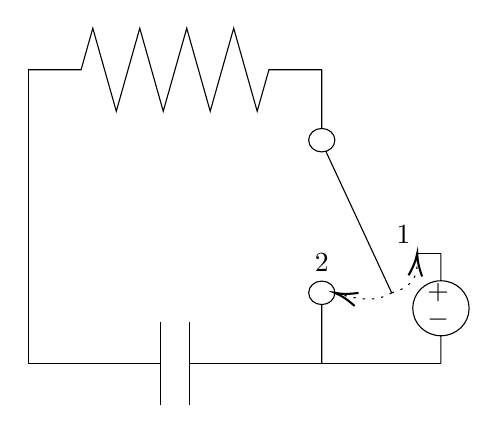
\begin{tikzpicture}[x=0.75pt,y=0.75pt,yscale=-1,xscale=1]
%uncomment if require: \path (0,504); %set diagram left start at 0, and has height of 504

%Shape: Resistor [id:dp30608216087842166] 
\draw   (150,80.58) -- (175.46,80.58) -- (181.11,60.58) -- (192.43,100.58) -- (203.74,60.58) -- (215.05,100.58) -- (226.37,60.58) -- (237.68,100.58) -- (248.99,60.58) -- (260.31,100.58) -- (265.97,80.58) -- (291.42,80.58) ;
%Straight Lines [id:da858527027889131] 
\draw    (150,80.58) -- (150,222) ;
%Shape: Capacitor [id:dp9610189215282299] 
\draw   (150,222) -- (213.64,222) (227.78,202) -- (227.78,242) (213.64,202) -- (213.64,242) (227.78,222) -- (291.42,222) ;
%Shape: Simple Switch [id:dp8738783462574553] 
\draw   (291.42,80.58) -- (291.42,108.86) (291.42,193.72) -- (291.42,222) (293.53,120.18) -- (325.11,188.06) (291.42,182.4) .. controls (294.91,182.4) and (297.74,184.93) .. (297.74,188.06) .. controls (297.74,191.18) and (294.91,193.72) .. (291.42,193.72) .. controls (287.93,193.72) and (285.11,191.18) .. (285.11,188.06) .. controls (285.11,184.93) and (287.93,182.4) .. (291.42,182.4) -- cycle (291.42,108.86) .. controls (294.91,108.86) and (297.74,111.4) .. (297.74,114.52) .. controls (297.74,117.64) and (294.91,120.18) .. (291.42,120.18) .. controls (287.93,120.18) and (285.11,117.64) .. (285.11,114.52) .. controls (285.11,111.4) and (287.93,108.86) .. (291.42,108.86) -- cycle ;
%Straight Lines [id:da2492031249151494] 
\draw    (348.84,222) -- (291.42,222) ;
%Shape: Output [id:dp8123576692630616] 
\draw   (348.84,182.25) .. controls (356.34,182.25) and (362.42,188.18) .. (362.42,195.5) .. controls (362.42,202.82) and (356.34,208.75) .. (348.84,208.75) .. controls (341.34,208.75) and (335.26,202.82) .. (335.26,195.5) .. controls (335.26,188.18) and (341.34,182.25) .. (348.84,182.25) -- cycle (348.84,169) -- (348.84,182.25) (348.84,222) -- (348.84,208.75) ;
%Straight Lines [id:da24217538064489208] 
\draw    (348.84,169) -- (337.42,169) ;
%Curve Lines [id:da8139879269218222] 
\draw  [dash pattern={on 0.84pt off 2.51pt}]  (325.11,188.06) .. controls (338.21,184.49) and (337.46,176.31) .. (337.38,171) ;
\draw [shift={(337.42,169)}, rotate = 94.82] [color={rgb, 255:red, 0; green, 0; blue, 0 }  ][line width=0.75]    (10.93,-3.29) .. controls (6.95,-1.4) and (3.31,-0.3) .. (0,0) .. controls (3.31,0.3) and (6.95,1.4) .. (10.93,3.29)   ;
%Curve Lines [id:da1445503769752734] 
\draw  [dash pattern={on 0.84pt off 2.51pt}]  (325.11,188.06) .. controls (320.2,190.88) and (314.48,192.84) .. (299.64,188.62) ;
\draw [shift={(297.74,188.06)}, rotate = 16.9] [color={rgb, 255:red, 0; green, 0; blue, 0 }  ][line width=0.75]    (10.93,-3.29) .. controls (6.95,-1.4) and (3.31,-0.3) .. (0,0) .. controls (3.31,0.3) and (6.95,1.4) .. (10.93,3.29)   ;

% Text Node
\draw (335.42,165.6) node [anchor=south east] [inner sep=0.75pt]    {$1$};
% Text Node
\draw (291.42,179) node [anchor=south] [inner sep=0.75pt]    {$2$};
% Text Node
\draw (341,182.4) node [anchor=north west][inner sep=0.75pt]    {$+$};
% Text Node
\draw (341,195.4) node [anchor=north west][inner sep=0.75pt]    {$-$};


\end{tikzpicture}

  \caption{Circuit Schematic}
  \label{fig:1}
\end{figure}

The switch flips between 1 and 2 based on a periodic cycle defined by a time interval $T$. Let us assume that a standard $1[\si{\micro\farad}]$ capacitor is used, along with a $100[\si{\ohm}]$ resistor. Furthermore, suppose that the battery has a voltage $V=5[\si{\volt}]$, and that, at time $t=0$, the switch has been in position $1$ for a long time, and is moved to $2$. We may begin by assuming that the initial voltage is entirely across the capacitor, such that:

$$V_o=5$$

According to discharging capacitors, we may write:

$$V=5e^{-\frac{t}{RC}}$$

for the stage in which the capacitor is losing charge. Let us start with a case in which the capacitor discharges to 25\% of its initial voltage value, and then the switch flips until fully charged (this repeats every $T$). This occurs when:

$$\ln\left( .01 \right)=-\frac{T}{RC}$$
$$T=-(100)(1\cdot10^{-6})\ln(.1)$$
$$T=.139[\si{\milli\second}]$$

Finally, let us assume that the plates are separated by $1[\si{\milli\meter}]$. Let us now proceed to the computational portion.

\newpage

\section{Computational Analysis}

\subsection{$T\to$ 25\% of Initial Voltage Discharge Time}

Using the scenario laid out in the preliminary assumptions, we may begin plotting. Let us choose a time step size of $t=10[\si{\micro\second}]$ and 100 iterations:

\begin{center}
  \begin{figure}[H]
    \centering
    \includegraphics[width=.9\textwidth]{Figures/QuarterT.png}
    \caption{Period ($T$) is Time to Discharge to $25\%$ Initial Voltage}
    \label{fig:2}
  \end{figure}
\end{center}

As expected, we can see the capacitor discharging in the long run, as it is unable to reach its initial value on recharge. Note that we do see the initial discharge fall to $25\%$ of the initial value ($5\to1.25[\si{\volt}]$).

\subsection{$T=20[\si{\micro\second}]$ (Small Period)}

Let us repeat the analysis with the same parameters specified in Section 2.1, but with a set period of $20[\si{\micro\second}]$. This yields:

\begin{figure}[H]
  \centering
  \includegraphics[width=.9\textwidth]{Figures/T20.png}
  \caption{Period of $20[\si{\micro\second}]$}
  \label{fig:3}
\end{figure}

We can see that, as compared to the initial period setting, this setting has oscillations occur much more frequently, as expected.

\subsection{Arbitrary $T$}

We can also test a case in which the oscillations occur randomly. That is, each interval for charge-discharge is randomly timed. We will set reasonable time boundaries so that the random time interval rests in the range $[2\cdot10^{-5},9.2\cdot10^{-4}]$. The following was generated:

\begin{figure}[H]
  \centering
  \includegraphics[width=.9\textwidth]{Figures/RandT.png}
  \caption{Random Period Value}
  \label{fig:4}
\end{figure}

\subsection{Edge Case Check}

We can confirm the accuracy of this projection by testing edge cases. Let us first see the capacitor discharge to $100\%$ of its initial value:

\begin{center}
  \begin{figure}[H]
    \centering
    \includegraphics[width=.9\textwidth]{Figures/NoDischarge.png}
    \caption{Discharge to $100\%$ (No Discharge)}
    \label{fig:4}
  \end{figure}
\end{center}

As expected, the switch never flips to position 2, which does not allow the capacitor to discharge. As expected, the voltage remains at its initial value. For the second edge case, we can see what happens when the capacitor discharges to $0\%$ of its initial value (no subsequent charge). This gives us:

\begin{center}
  \begin{figure}[H]
    \centering
    \includegraphics[width=.9\textwidth]{Figures/OnlyDischarge.png}
    \caption{Discharge to $0\%$ (No Charge After Discharge)}
    \label{fig:5}
  \end{figure}
\end{center}

As expected, we can see that the capacitor simply discharges.

\section{Conclusion}

As such, we are successfully able to model oscillating capacitors with the attached code (see Appendix).

\newpage

\section{Appendix}

\lstinputlisting[
    caption=GNU Octave Code, % Caption above the listing
	label=lst:L1, % Label for referencing this listing
	language=matlab, % Use python functions/syntax highlighting
	frame=single, % Frame around the code listing
	showstringspaces=false, % Don't put marks in string spaces
	numbers=left, % Line numbers on left
	numberstyle=\tiny, % Line numbers styling
    backgroundcolor=\color{black!5}, % Set background color
    keywordstyle=\color{magenta!80}, % Set keyword color
    commentstyle=\color{blue!80}, % Set comment color
    stringstyle=\color{green!80}, % Set string color
    breaklines=true
  ]{HWC.m}



\end{document}

